\makeheading{Lecture 12 | 2020-10-21}
\section{Multicollinearity}
Multicollinearity: occurs when some explanatory
variables have a \textbf{strong linear}
relationship amongst themselves. For example,
this might occur exactly
\[ \symbf{x}_3=\alpha_0\symbf{1}+\alpha_1\symbf{x}_1+\alpha_2\symbf{x}_2 \]
in which case the columns of $ X $ would be \textbf{linearly dependent}
and $ X^\top X $ does not have an inverse. Practically,
there is no new info including $ \symbf{x}_3 $
when $ \symbf{x}_1,\symbf{x}_2 $ are in the model.
\textbf{Approximately},
\[ \symbf{x}_3\approx \alpha_0\symbf{1}+\alpha_1\symbf{x}_1+\alpha_2\symbf{x}_2 \]
in which case the columns of $ X $ are close to being
linearly dependent which cases $ \Var{\hat{\beta}_j} $
to be \textbf{inflated}, in turn leads to inaccurate confidence
intervals and conclusions of hypothesis tests
for the regression parameters, in practice.
$ \Se{\hat{\beta}_j} $ when fitting models can change drastically
when adding/removing variables from the model.

\begin{Example}{Hockey (NHL)}{}
    In the NHL we have $ \text{Goals}+\text{Assists}=\text{Points} $.
    Suppose we want to predict a forward's salary. Define
    \begin{itemize}
        \item $ x_1= $ Goals
        \item $ x_2= $ Assists
        \item $ x_3= $ Points
    \end{itemize}
    $ x_3=x_1+x_2 $, therefore we have exact multicollinearity.
\end{Example}
\begin{Example}{Burmese Pythons in Florida (2017)}{}
    \begin{itemize}
        \item $ y= $ fat content
        \item $ x_1= $ mass
        \item $ x_2= $ overall length
        \item $ x_3= $ snout-to-vent length
    \end{itemize}
    It turns out that $ x_2 $ and $ x_3 $ are highly
    correlated. Including all variables in
    regression lead to inflated $ \Se{\hat{\beta}_2} $
    and $ \Se{\hat{\beta}_3} $.
\end{Example}

\section{Detection of Multicollinearity}
If two predictors are related
\begin{itemize}
    \item Scatter plot matrix [all possible pairs of
                  scatter plots b/w $ y,x_1,x_2,\ldots,x_p $]
    \item Correlation matrix (all pairwise correlations)
\end{itemize}
\begin{Definition}{Variance inflation factor}{}
    For multicollinearity between more than two
    predictors, we can define the \textbf{variance inflation factor}
    (VIF).
    \[ \VIF_j=\frac{\Var{\hat{\beta}_j}}{\Var{\hat{\beta}_j^*}} \]
    for $ j=1,\ldots,p $,
    where $ \hat{\beta}_j $ is the estimate of $ \beta_j $ with all predictors
    in the model, and $ \hat{\beta}_j^* $ estimate
    of $ \beta_j $ based on regression with $ x_j $ only.
\end{Definition}
\begin{Theorem}{}{}
    \[ \VIF_j\geqslant 1 \]

\end{Theorem}
Fit multiple linear regression model of $ x_j $ in terms of other predictors;
that is,
\[ x_{i j}=\alpha_0+\alpha_1x_{i1}+\cdots+\alpha_{j-1}x_{i(j-1)}+
    \alpha_{j+1}x_{i(j+1)}+\cdots+\alpha_p x_{i p}+\varepsilon_{ij} \]
and compute $ R^2 $ for this model, call it $ R_j^2 $.

Intuition: if $ R_j^2 $ is close to 1, $ x_j $ is strongly
related linearly to other predictors. It can be shown that
\[ \VIF_j=\frac{1}{1-R_j^2}  \]
If $ \VIF_j\ge 10 $, then there is solid evidence of multicollinearity;
that is, $ R_j^2>0.9 $.

Procedure:
\begin{itemize}
    \item remove predictors with largest $ \VIF $, if it exceeds 10.
          Repeat until no more multicollinearity.
\end{itemize}
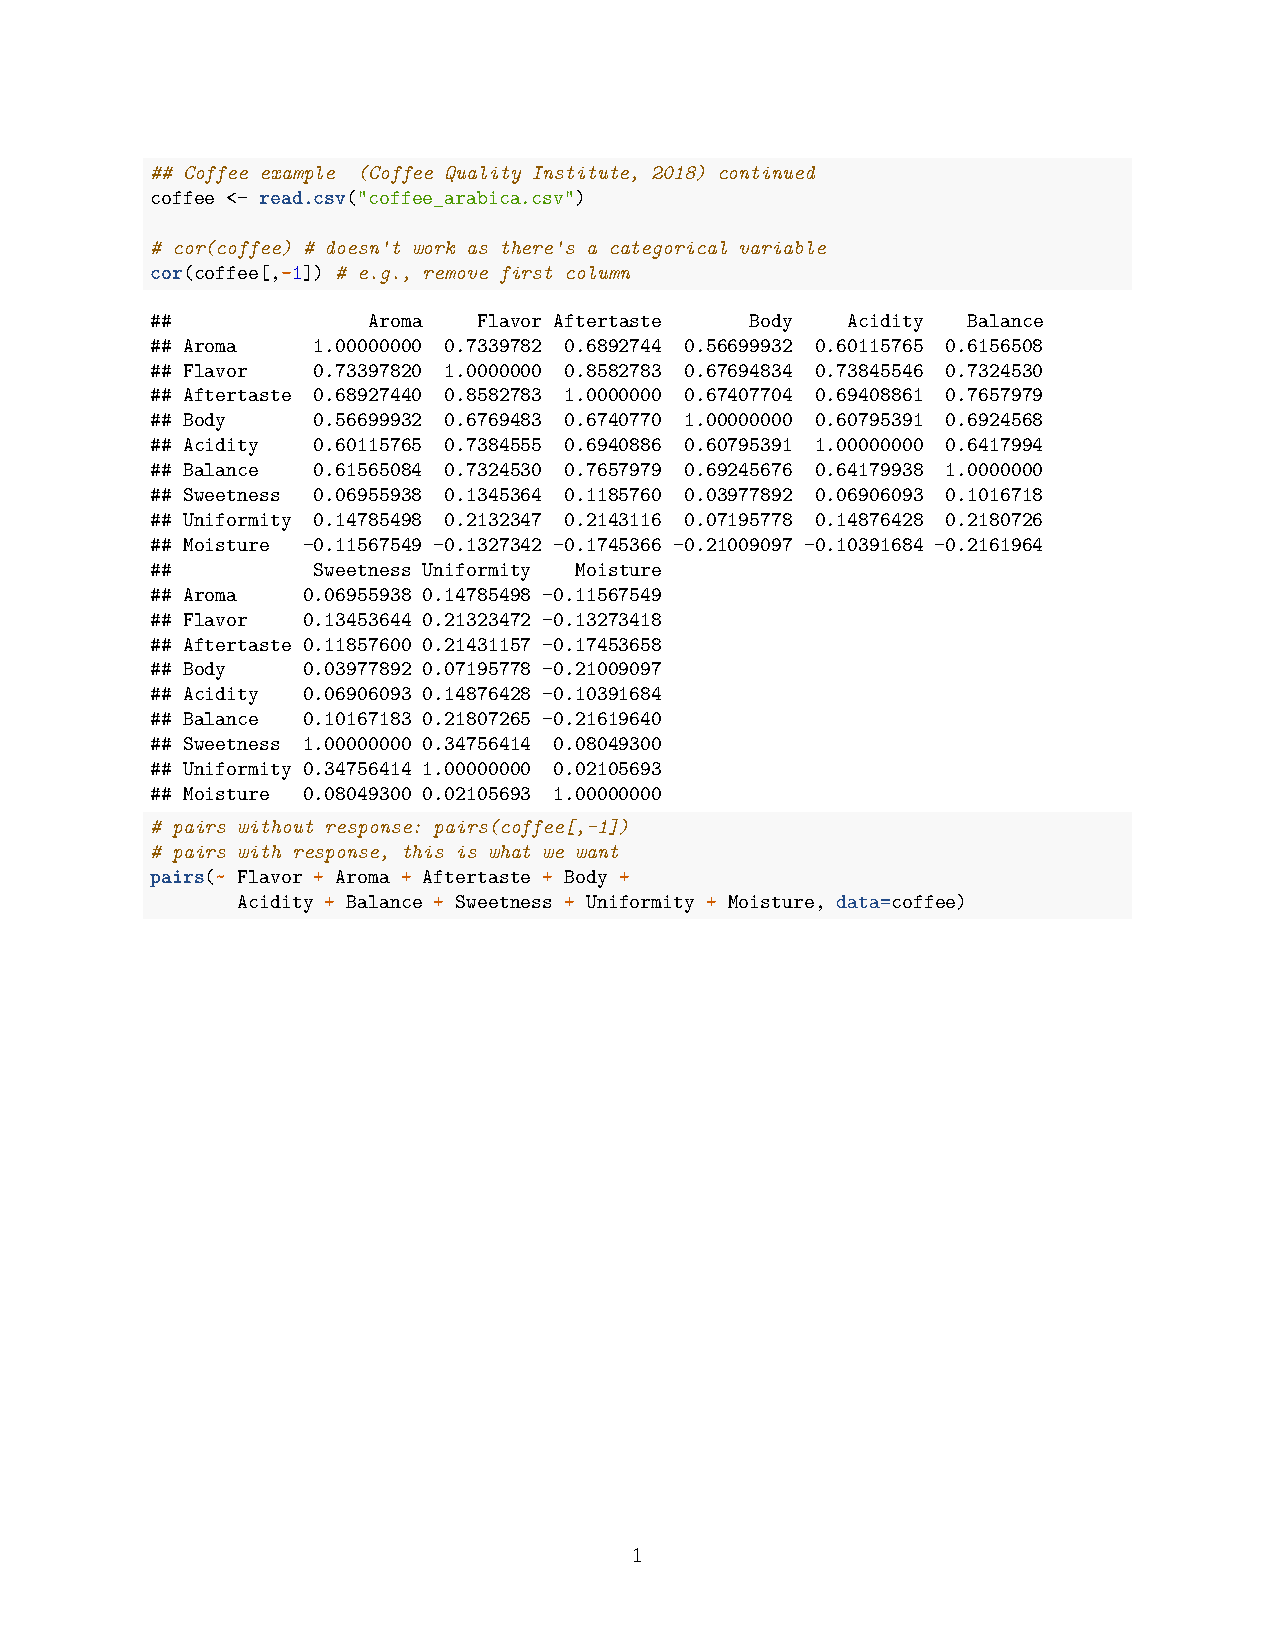
\includepdf[pages=-]{multicollinear-demo}
